\documentclass[xcolor={dvipsnames},8pt]{beamer}
\title[V\'{i}tor Costa]{The Public-Private Wage Gap in Brazil:\\ new evidence from administrative data}
\author[RA Progress Report - Wage Gap Project]{V\'{i}tor Costa}
\date{November 2018}
\usefonttheme{structuresmallcapsserif}
\usetheme{Madrid}
\usecolortheme{beaver}
\setbeamertemplate{navigation symbols}{}
\setbeamertemplate{footline}{
  \leavevmode%
  \hbox{%
  \begin{beamercolorbox}[wd=.5\paperwidth,ht=2.25ex,dp=1ex,center]{author in head/foot}%
    \usebeamerfont{author in head/foot}\insertshortauthor
  \end{beamercolorbox}%
  \begin{beamercolorbox}[wd=.5\paperwidth,ht=2.25ex,dp=1ex,center]{title in head/foot}%
    \usebeamerfont{title in head/foot}\qquad \insertshorttitle \qquad\qquad\qquad \insertframenumber
  \end{beamercolorbox}}%
  \vskip0pt%
}

%
\setbeamertemplate{caption}{\raggedright\insertcaption\par}
\usepackage{pdflscape, graphicx, booktabs, dcolumn, listings, amsmath,bbm,courier,pgffor,fixltx2e, natbib,enumerate,amssymb,amsfonts,color,hyperref,array,calc,multirow,tikz,amsthm,anyfontsize,bbm}

\usepackage[section]{placeins}
\usepackage[english]{babel}
\usepackage[justification=centering]{caption}
\captionsetup{labelformat=empty}
\usepackage[flushleft]{threeparttable}
\newtheorem{findings}[theorem]{Findings}
\usepackage[T1]{fontenc}
\usepackage{lmodern}
\usepackage[percent]{overpic}
\usepackage{setspace}
\setstretch{1.5}

\newtheorem{prop}{\protect\propositionname}
\addto\captionsamerican{\renewcommand{\propositionname}{Proposition}}
\addto\captionsenglish{\renewcommand{\propositionname}{Proposition}}
\providecommand{\propositionname}{Proposition}
\setbeamertemplate{theorems}[numbered]
\theoremstyle{definition}
\newtheorem*{theorem*}{Definition}

\RequirePackage{ifthen}
\newboolean{sectiontoc}

\AtBeginSection[]{
\begin{frame}[plain]{Outline}
\ifthenelse{\boolean{sectiontoc}}{\tableofcontents[]}{\tableofcontents[currentsection]}
\addtocounter{framenumber}{-1}
\end{frame}}

\newcommand{\firstsection}[1]{\setboolean{sectiontoc}{true} \section{#1} \setboolean{sectiontoc}{false}}
\newcommand{\indep}{\mathrel{\text{\scalebox{1.07}{$\perp\mkern-10mu\perp$}}}}


\setbeamercolor{button}{bg=structure.fg,fg=white}

\setbeamertemplate{library}[text]

\begin{document}

\begin{frame}[plain]
\titlepage
\addtocounter{framenumber}{-1}
\end{frame}

\begin{frame}{Motivation}
\begin{itemize}
    \item Wage differentials seem to be in favor of public sector employees in both developed and developing countries.
    \item The public sector premium aggravates income inequality
    \begin{itemize}
        \item Brazilian Gini would be 3\% lower \citep{Souza2013}
        \item Government employs up to 100\% of formal workers at municipal level
    \end{itemize}
    \item Big dispersion in estimates for the Brazilian case.
    \begin{itemize}
        \item From 0\% \citep{Emilio2012} 
        \item to 270\% \citep{Tenoury2017}  
    \end{itemize}
    \item RAIS allows for better treatment of endogeneity.
    \begin{itemize}
        \item Larger $T$: 13 years in our sample.
        %\item \color{red} How does my approach compare to the Heckman Selection? \color{black}
    \end{itemize}
\end{itemize}
\end{frame}


\begin{frame}{Research Questions}

\begin{itemize}
    \item Is there a public sector wage premium across individuals with similar characteristics?\\ 
    \item How does this gap change along the wage distribution?\\
    \item What happens to specific demographic groups?\\
    \item How do results change when endogenous selection is taken into account? 
\end{itemize}
\end{frame}

\begin{frame}{Data}
 
\begin{itemize}
    \item RAIS is a matched employer-employee database
    \item Employers have high incentive to comply
    \item It has universal coverage of the Brazilian formal labor market
\end{itemize}

\end{frame}

\begin{frame}{Descriptive Statistics}

\begin{itemize}
    \item 
\end{itemize}
\end{frame}

\begin{frame}{(Quantile) Oaxaca-Blinder Decomposition}
Conditional on a set $X_{it}$ of observed individual characteristics, expected wage $y_{it}$ is given by
\begin{align*}
    y_{it}^{1} = X_{it}^{1}\beta^{1}+u_{it}\\
    y_{it}^{0} = X_{it}^{0}\beta^{0}+u_{it}
\end{align*}
which can be rewritten as
\begin{align*}
    \bar{y}_{t}^{1} - \bar{y}_{t}^{0} &= \bar{X}_{t}^{1}\beta^{1} -\bar{X}_{t}^{0}\beta^{0} \\
    &= \underbrace{\left(\bar{X}_{t}^{1}-\bar{X}_{t}^{0}\right)\beta^{0}}_{Characteristics} +\underbrace{\bar{X}_{t}^{1}\left(\beta^{1}-\beta^{0}\right)}_{Structural}
\end{align*}
\begin{itemize}
    \item Quantile Oaxaca-Blinder from \citep{Chernozhukov2013} 
    \item Self-selection treatment from \citep{Canay2011}, FE's are just shifters
\end{itemize}
\end{frame}

\begin{frame}{Worker Fixed Effects}
\tiny{
\begin{align*}
    log(hourly.wage)_{it} =& a_i + region_{it} + year_t + \\
     &\beta_1*tenure_{it} + \beta_2*tenure^2_{it} + \beta_3*med\_skill_{it} + \beta_4*high\_skill_{it} + u_i
\end{align*}}%

\begin{figure}[h]
    \centering
    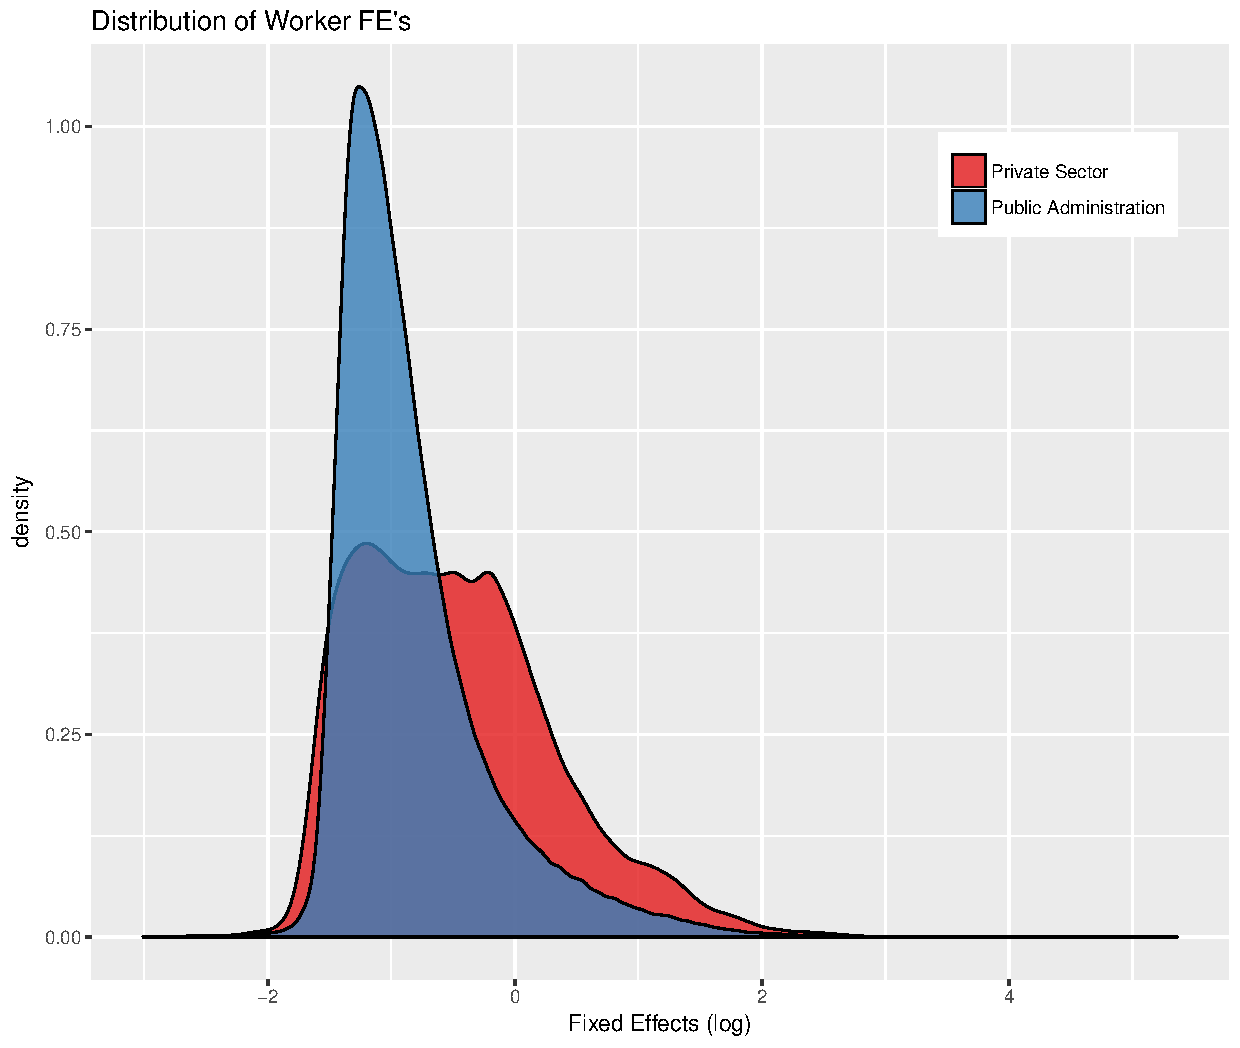
\includegraphics[scale = 0.32]{graphs/001_fe_onepc.pdf}
\end{figure}
\end{frame}

\begin{frame}{Wage Gap Over the Years}
\begin{figure}[h]
    \centering
    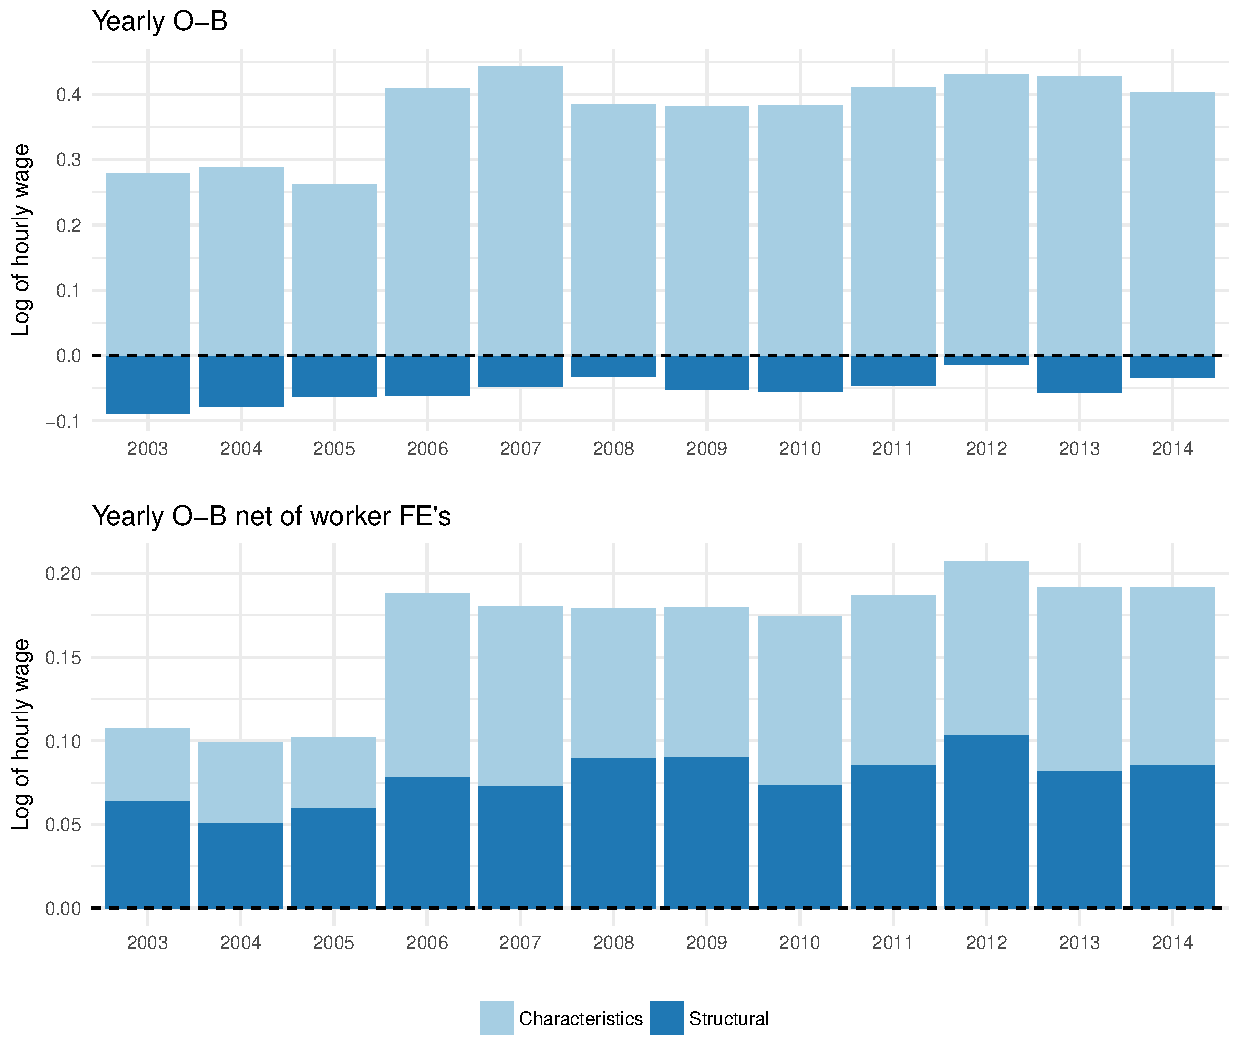
\includegraphics[scale = 0.45]{graphs/002_yearly_ob_onepc.pdf}
\end{figure}
\end{frame}

\begin{frame}{Quantile Oaxaca-Blinder Decomposition}
\begin{figure}[h]
    \centering
    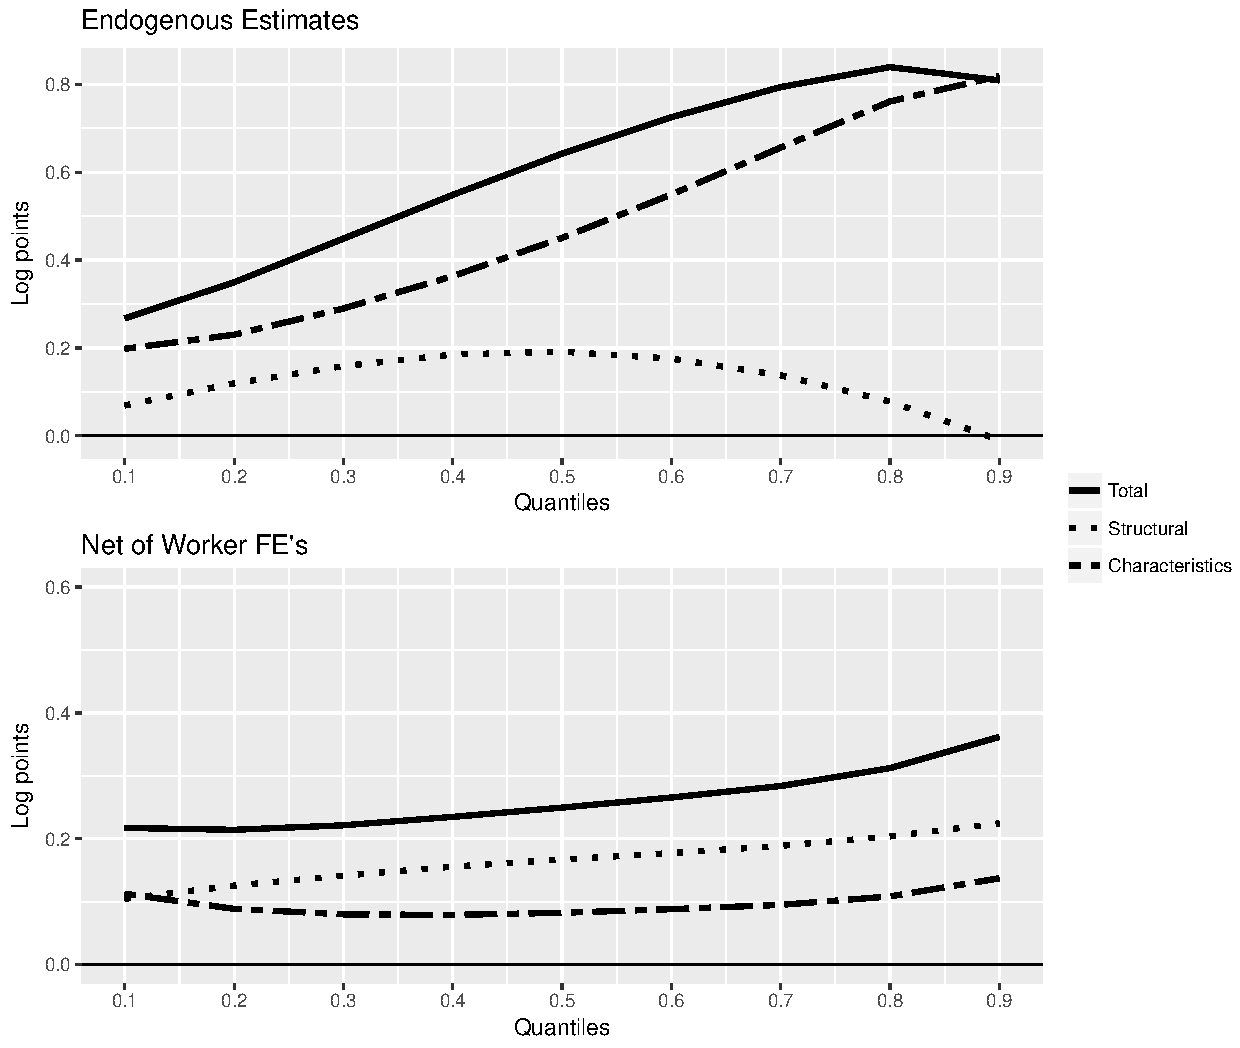
\includegraphics[scale = 0.45]{graphs/003_qob_debug.pdf}
\end{figure}
\end{frame}

\begin{frame}{QOB by Sex and Skill}

\begin{figure}[h]
    \centering
    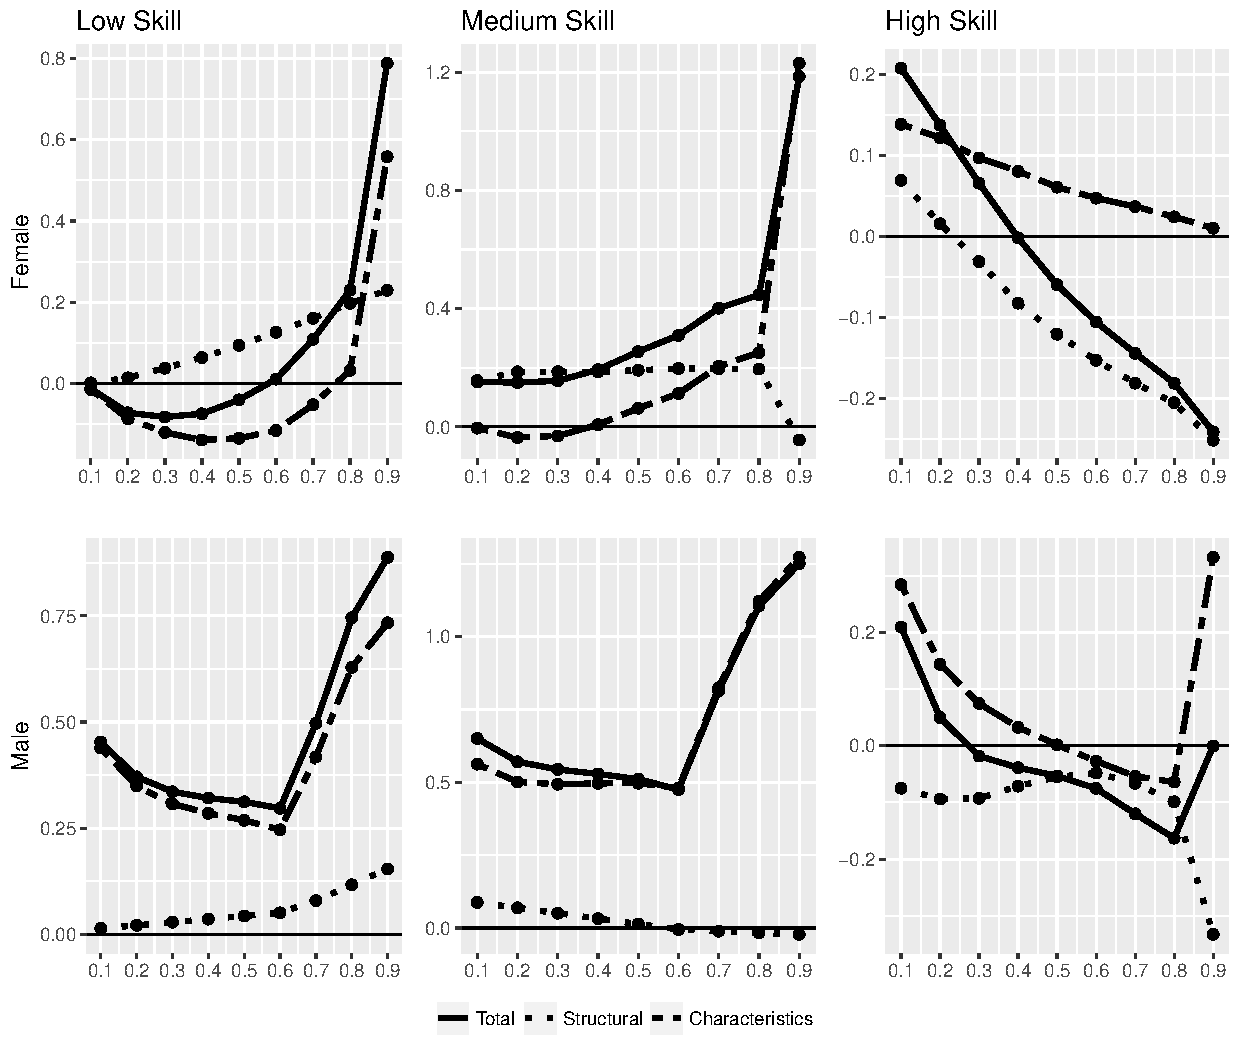
\includegraphics[scale = 0.45]{graphs/003_qob_gs_debug.pdf}
\end{figure}

\end{frame}

\begin{frame}{QOB by Race and Skill}

\begin{figure}[h]
    \centering
    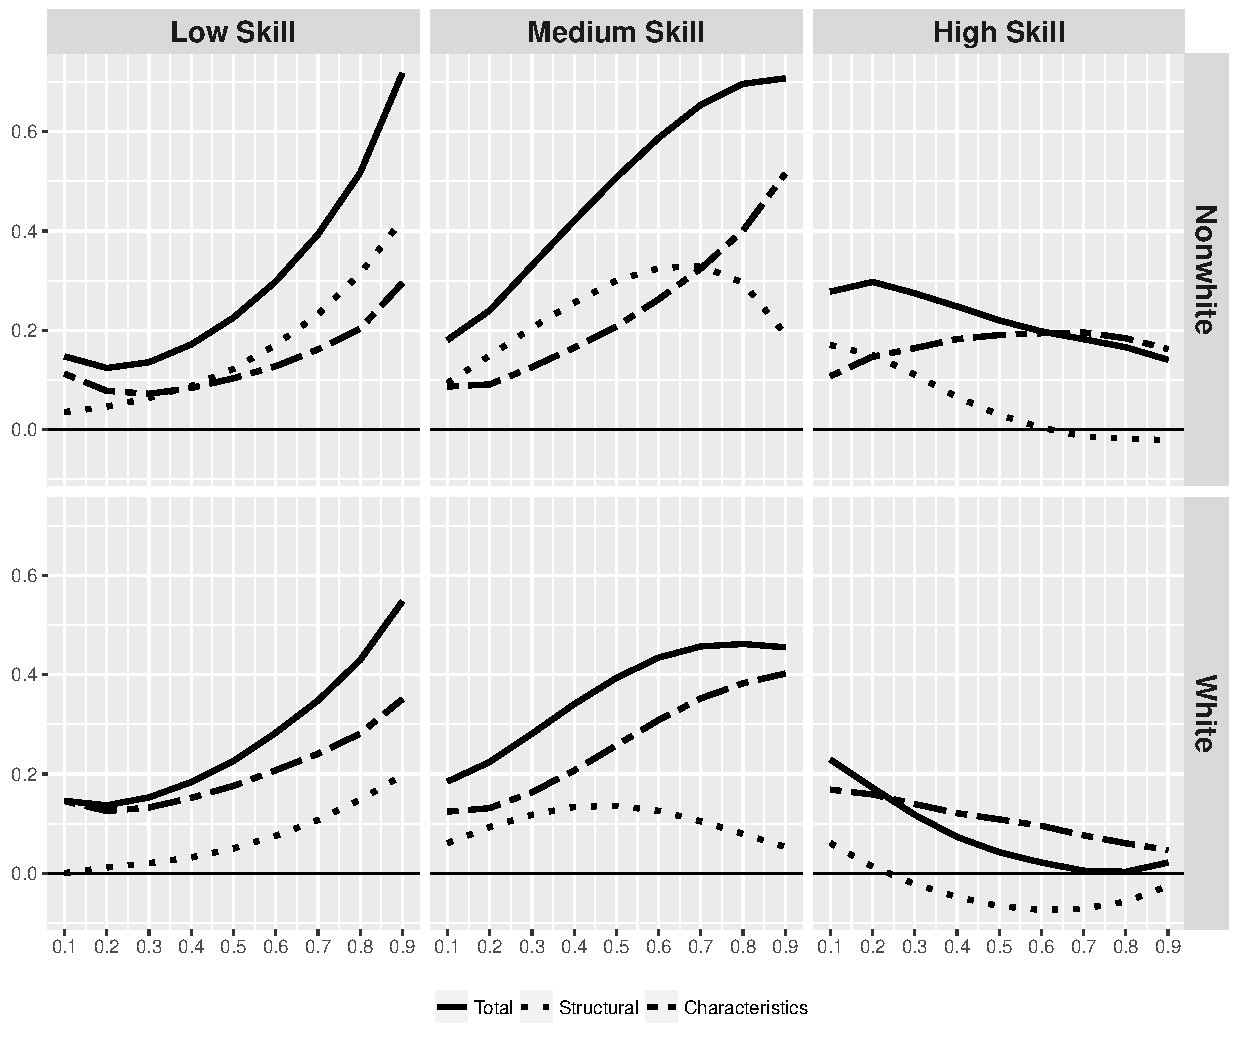
\includegraphics[scale = 0.45]{graphs/003_qob_rs_debug.pdf}
\end{figure}

\end{frame}

%\begin{frame}{Preliminary Conclusions}
%
%\begin{itemize}
%    \item 
%\end{itemize}
%\end{frame}

\begin{frame}[allowframebreaks*] %allow to expand references to multiple frames (slides)
\frametitle{References}
\scriptsize{\bibliographystyle{chicago}}
\bibliography{library} %bibtex file name without .bib extension
\end{frame}

\end{document}
